\begin{frame}{Inducing Inputs}
	The graphical model for the gaussian process regression looks like this.
	\begin{figure}[!h]
		\centering
		\subfloat{
			\scalebox{0.5}{
				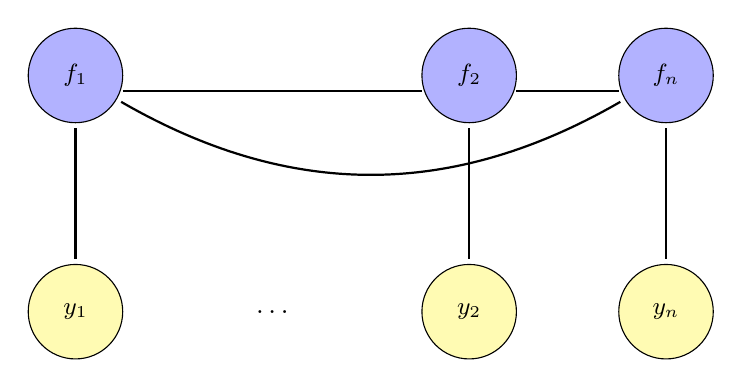
\begin{tikzpicture}
	\tikzstyle{x_i} = [circle, draw, fill=green!50, minimum size=1.2cm, text width=0.8cm, align=center, font=\large]
\tikzstyle{f_i} = [circle, draw, fill=blue!30, minimum size=1.2cm, inner sep=2pt, outer sep=2pt, font=\small, align=center]
\tikzstyle{y_i} = [circle, draw, fill=yellow!30, minimum size=1.2cm, inner sep=2pt, outer sep=2pt, font=\small, align=center]
\tikzstyle{edge_label} = [font=\small, label={[label distance = -4pt]90:$\text$}]
\tikzstyle{edge} = [thick, >=stealth]
\tikzstyle{biedge} = [thick, >=stealth]
\def\step{-3}
\def\layerpos{3}

% %data points
% \foreach \name/\x in {x_1/-2.5, x_2/2.5, x_n/5} 
%   	\node[x_i] (\name) at (\x, \layerpos) {$\name$};

% \node (other^1_1) at (0, \layerpos) {$\ldots$};

%latent process values
% \pgfmathsetmacro{\layerpos}{\layerpos + \step}

\foreach \name/\x in {f_1/-2.5, f_2/2.5, f_n/5} 
  	\node[f_i] (\name) at (\x, \layerpos) {$\name$};

% \node (other^2) at (0, \layerpos) {$\ldots$};
% \foreach \from/\to in {x_1/f_1, x_2/f_2, x_n/f_n}
% 	\draw[edge] (\from) -- (\to);

\draw[biedge] (f_1)++(0.6,-0.2) -- ++(3.8,0); %(f_2);
\draw[biedge] (f_2)++(0.6,-0.2) -- +(1.3,0);% ++ (f_n);
\draw [biedge] (f_1) to [out=-30,in=-150] (f_n);

%observables
\pgfmathsetmacro{\layerpos}{\layerpos + \step}

\foreach \name/\x in {y_1/-2.5, y_2/2.5, y_n/5} 
  	\node[y_i] (\name) at (\x, \layerpos) {$\name$};

\node (other^3) at (0, \layerpos) {$\ldots$};
\foreach \from/\to in {f_1/y_1, f_2/y_2, f_n/y_n}
	\draw[edge] (\from) -- (\to);
\end{tikzpicture}


			}
		}
	\end{figure}
\end{frame}

\begin{frame}{Inducing Inputs}
	Now we slightly change the model, adding a set of latent variables $u$.
	\begin{figure}[!h]
		\centering
		\subfloat{
			\scalebox{0.5}{
				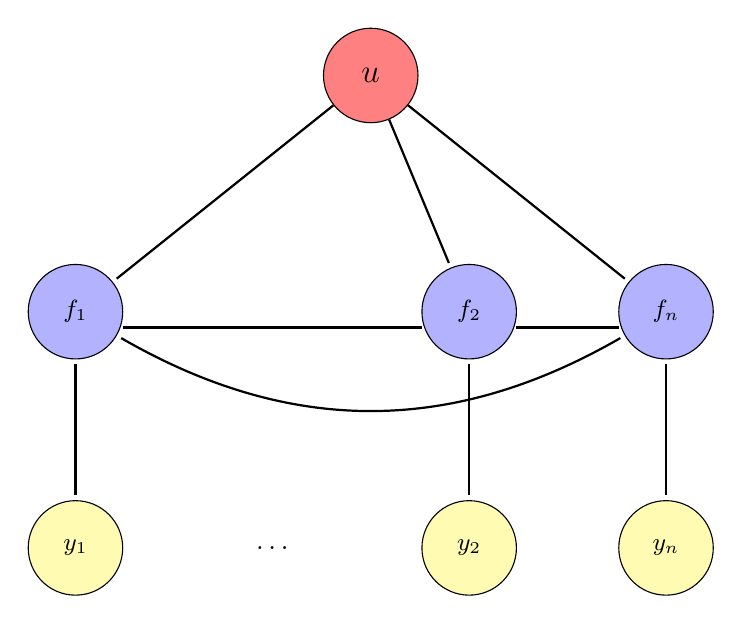
\begin{tikzpicture}
	\tikzstyle{u} = [circle, draw, fill=red!50, minimum size=1.2cm, text width=0.8cm, align=center, font=\large]
	\tikzstyle{x_i} = [circle, draw, fill=green!50, minimum size=1.2cm, text width=0.8cm, align=center, font=\large]
\tikzstyle{f_i} = [circle, draw, fill=blue!30, minimum size=1.2cm, inner sep=2pt, outer sep=2pt, font=\small, align=center]
\tikzstyle{y_i} = [circle, draw, fill=yellow!30, minimum size=1.2cm, inner sep=2pt, outer sep=2pt, font=\small, align=center]
\tikzstyle{edge_label} = [font=\small, label={[label distance = -4pt]90:$\text$}]
\tikzstyle{edge} = [thick, >=stealth]
\tikzstyle{biedge} = [thick, >=stealth]
\def\step{-3}
\def\layerpos{3}

% %data points
% \foreach \name/\x in {x_1/-2.5, x_2/2.5, x_n/5} 
%   	\node[x_i] (\name) at (\x, \layerpos) {$\name$};

% \node (other^1_1) at (0, \layerpos) {$\ldots$};

%latent process values
% \pgfmathsetmacro{\layerpos}{\layerpos + \step}

\foreach \name/\x in {f_1/-2.5, f_2/2.5, f_n/5} 
  	\node[f_i] (\name) at (\x, \layerpos) {$\name$};

% \node (other^2) at (0, \layerpos) {$\ldots$};
% \foreach \from/\to in {x_1/f_1, x_2/f_2, x_n/f_n}
% 	\draw[edge] (\from) -- (\to);

\draw[biedge] (f_1)++(0.6,-0.2) -- ++(3.8,0); %(f_2);
\draw[biedge] (f_2)++(0.6,-0.2) -- +(1.3,0);% ++ (f_n);
\draw [biedge] (f_1) to [out=-30,in=-150] (f_n);

%observables
\pgfmathsetmacro{\layerpos}{\layerpos + \step}

\foreach \name/\x in {y_1/-2.5, y_2/2.5, y_n/5} 
  	\node[y_i] (\name) at (\x, \layerpos) {$\name$};

\node (other^3) at (0, \layerpos) {$\ldots$};
\foreach \from/\to in {f_1/y_1, f_2/y_2, f_n/y_n}
	\draw[edge] (\from) -- (\to);
	\pgfmathsetmacro{\layerpos}{\step/2}
	\node[u] (inputs) at (1.25, 6) {$u$};

	\foreach \to in {f_1, f_2, f_n}
		\draw[edge] (inputs) -- (\to);
\end{tikzpicture}


			}
		}
	\end{figure}
	The joint probability of latent and observable variables now is given by
	$$p(y, f, u) = p(y | f) p(f | u) p(u).$$
\end{frame}

\begin{frame}{Inducing Inputs}
	The latent variables $u$ are referred to as inducing inputs. The intuition behind them is that they are considered as the values of the process at new data points $z_1, \ldots, z_m$. We will have to introduce some more notation now.

	\begin{itemize}
		\item $Z_m \in \R^{m \times d}$ — the matrix, comprised of the coordinates of the inducing inputs inputs $z_1, \ldots, z_m$.
		\item $K_{nn} = K(X, X)$
		\item $K_{mm} = K(Z_m, Z_m)$
		\item $K_{mn} = K(Z_m, X)$
		\item $K_{nm} = K(X, Z_m) = K_{mn}^T$ 
	\end{itemize}
	As $u_i$ are considered to be generated from the same gaussian process, as $f_i$, we have the following formulas.
	$$p(u) = \N(u|0, K_{mm}),$$
	$$p(f|u) = \N (f|K_{nm} K_{mm}^{-1}u, \tilde K),$$
	where $\tilde K = K_{nn} - K_{nm} K_{mm}^{-1} K_{mn}.$
\end{frame}

\begin{frame}{Evidence Lower Bound}
	The standard variational lower bound for the marginal likelihood $p(y)$ for our augmented model is
	$$\log p(y) \ge \E_{q(u, f)} \log \frac {p(y, u, f)}{q(u, f)} = \E_{q(u, f)}\log p(y | f) - \KL{q(u, f)} {p(u, f)}.$$

	Our model implies $\E_{q(u, f)} \log p(y | f) = \E_{q(f)} \log p(y | f)$, where $q(f)$ is the marginal of $q(u, f)$.

	We will consider the variational distributions of the following form:
	$$q(u, f) = p(f | u) q(u),$$
	where $q(u) \sim \N(u|\mu, \Sigma)$. This implies $q(f)$
	$$q(f) = \int p(u | f) q(u) du = $$
	$$\N(f| K_{nm} K_{mm}^{-1} \mu, K_{nn} + K_{nm} K_{mm}^{-1}(\Sigma - K_{mm}) K_{mm}^{-1} K_{mn}).$$
\end{frame}

\begin{frame}{Evidence Lower Bound}
	Now, consider the KL-divergence in the lower bound we've devised.
	$$\KL{q(u, f)} {p(u, f)} = \KL{q(u) p(f|u)} {p(u) p(f|u)} = \KL{q(u)} {p(u)}.$$

	Finally, the lower bound is
	$$\log p(y) \ge \E_{q(f)} \log p(y | f) - \KL{q(u)} {p(u)} = $$ $$ = \sum_{i = 1}^{n} \E_{q(f_i)} \log p(y_i | f_i) - \KL{q(u)} {p(u)}.$$

	Note, that although, we've devised this bound for the regression problem, we never used the fact, that we are actually performing regression. This bound holds for binary classification problem as well.

	However, in the case of GP-regression, the right-hand side of the bound can be computed analytically in a closed form.
\end{frame}

\begin{frame}{SVI method}
	Substituting the normal distributions $q(u)$, $p(u)$, $q(f)$ and $p(y|f)$ back into the lower bound, we obtain the following inequality.
	$$\log p(y) \ge \sum_{i = 1}^{n} \left( \log \N(y_i | k_i^T K_{mm}^{-1} \mu, \sigma_n^2) - \frac 1 {2 \sigma_n^2} \tilde K_{ii} - \frac 1 2 \tr (\Sigma \Lambda_i) \right) - $$
	$$ -\frac 1 2 \left (\log \frac {|K_{mm}|} {|\Sigma|} - m + \tr(K_{mm}^{-1} \Sigma) + \mu^T K_{mm}^{-1} \mu \right),$$
	where $\Lambda_i = \frac 1 {\sigma_n^2} K_{mm}^{-1} k_i k_i^T K_{mm}^{-1}$, and $k_i$ is the $i$-th column of the matrix $K_{mn}$.

	This lower can be maximized with respect to kernel hyper-parameters and variational parameters $\mu, \Sigma$ using the stochastic optimization techniques. The method was proposed at [Hensman et al., 2013]. The authors suggest using the stochastic gradient descent with natural gradients for variational parameters. The complexity of computing a stochastic update for one object is $O(m^3)$.
\end{frame}

\begin{frame}{Titsias's method}
	The lower bound we devised can also be maximized with respect to variational parameters analytically, which was suggested in [Titsias, 2009]. The optimal distribution is $q^*(u) \sim \N(u|\hat u, \Lambda^{-1})$, where
	$$\Lambda = \frac 1 {\sigma_n^2} K_{mm}^{-1} K_{mn} K_{nm} K_{mm}^{-1} + K_{mm}^{-1},$$
	$$\hat u = \frac 1 {\sigma_n^2} \Lambda^{-1} K_{mm}^{-1} K_{mn} y.$$
	Substituting this distribution back to the ELBO, we obtain
	$$\log p(y) \ge -\frac 1 2 \left(n \log 2\pi + \log |B| + y^T B^{-1} y + \frac 1 {\sigma_n^2} \tr(\tilde K)\right),$$
	where $B = \sigma_n^2 I + K_{nm} K_{mm}^{-1} K_{mn}$. The complexity of computing the optimal distribution parameters, the lower bound and it's gradients is $O(n m^2)$. However, we can not apply stochastic optimization in this case.
\end{frame}

\begin{frame}{Example}
	\begin{figure}[!h]
		\centering
		\subfloat{
			\scalebox{0.5}{
				\input{../../Code/Experiments/pictures/1dgp-regression_means.pgf}
			}
		}
		\subfloat{
			\scalebox{0.5}{
				\input{../../Code/Experiments/pictures/1dgp-regression_vi.pgf}
			}
		}
		\caption{Example of two implementations of the Titsias's method. The \lstinline{vi} method maximizes the lower bound with respect to the positions of inducing inputs, while the \lstinline{means} method just uses the K-means cluster centers as inducing point positions.}
	\end{figure}
\end{frame}